\section{Le Méta-Modèle Cinématique}
Le métamodèle cinématique est organisé autour de trois principaux packages:
\begin{itemize}
  \item \textbf{Toolkit}: représente les concepts liés à la définition des widgets\footnote{Elément visuel d'une interface graphique (bouton, ascenseur,liste déroulante, etc\dots)} \textsc{ihm}.

Le package Toolkit est construit de la manière suivante:

\begin{figure}[htb]
  \centering
  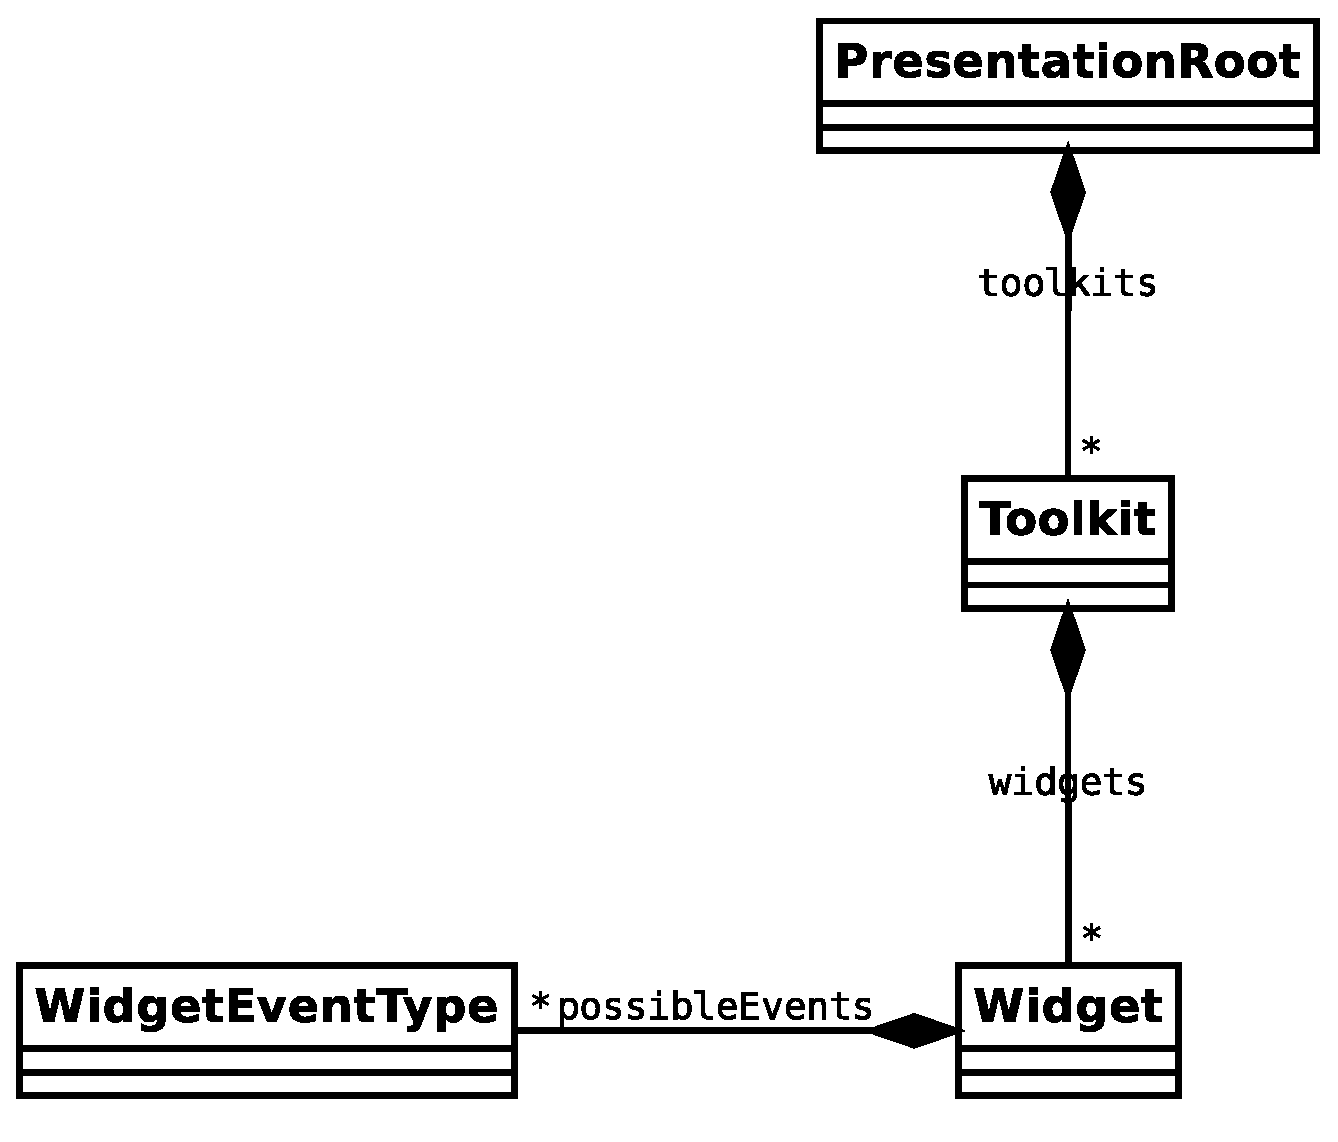
\includegraphics[scale=.3]{img/toolkit.eps}
  \caption{Métamodèle toolkit}
  \label{fig:toolkit}
\end{figure}
  \item \textbf{View}: représente les concepts liés à la définition des écrans \textsc{ihm}.

La construction du package View est illustrée sur la figure \ref{fig:view}.
\begin{figure}[H]
  \centering
  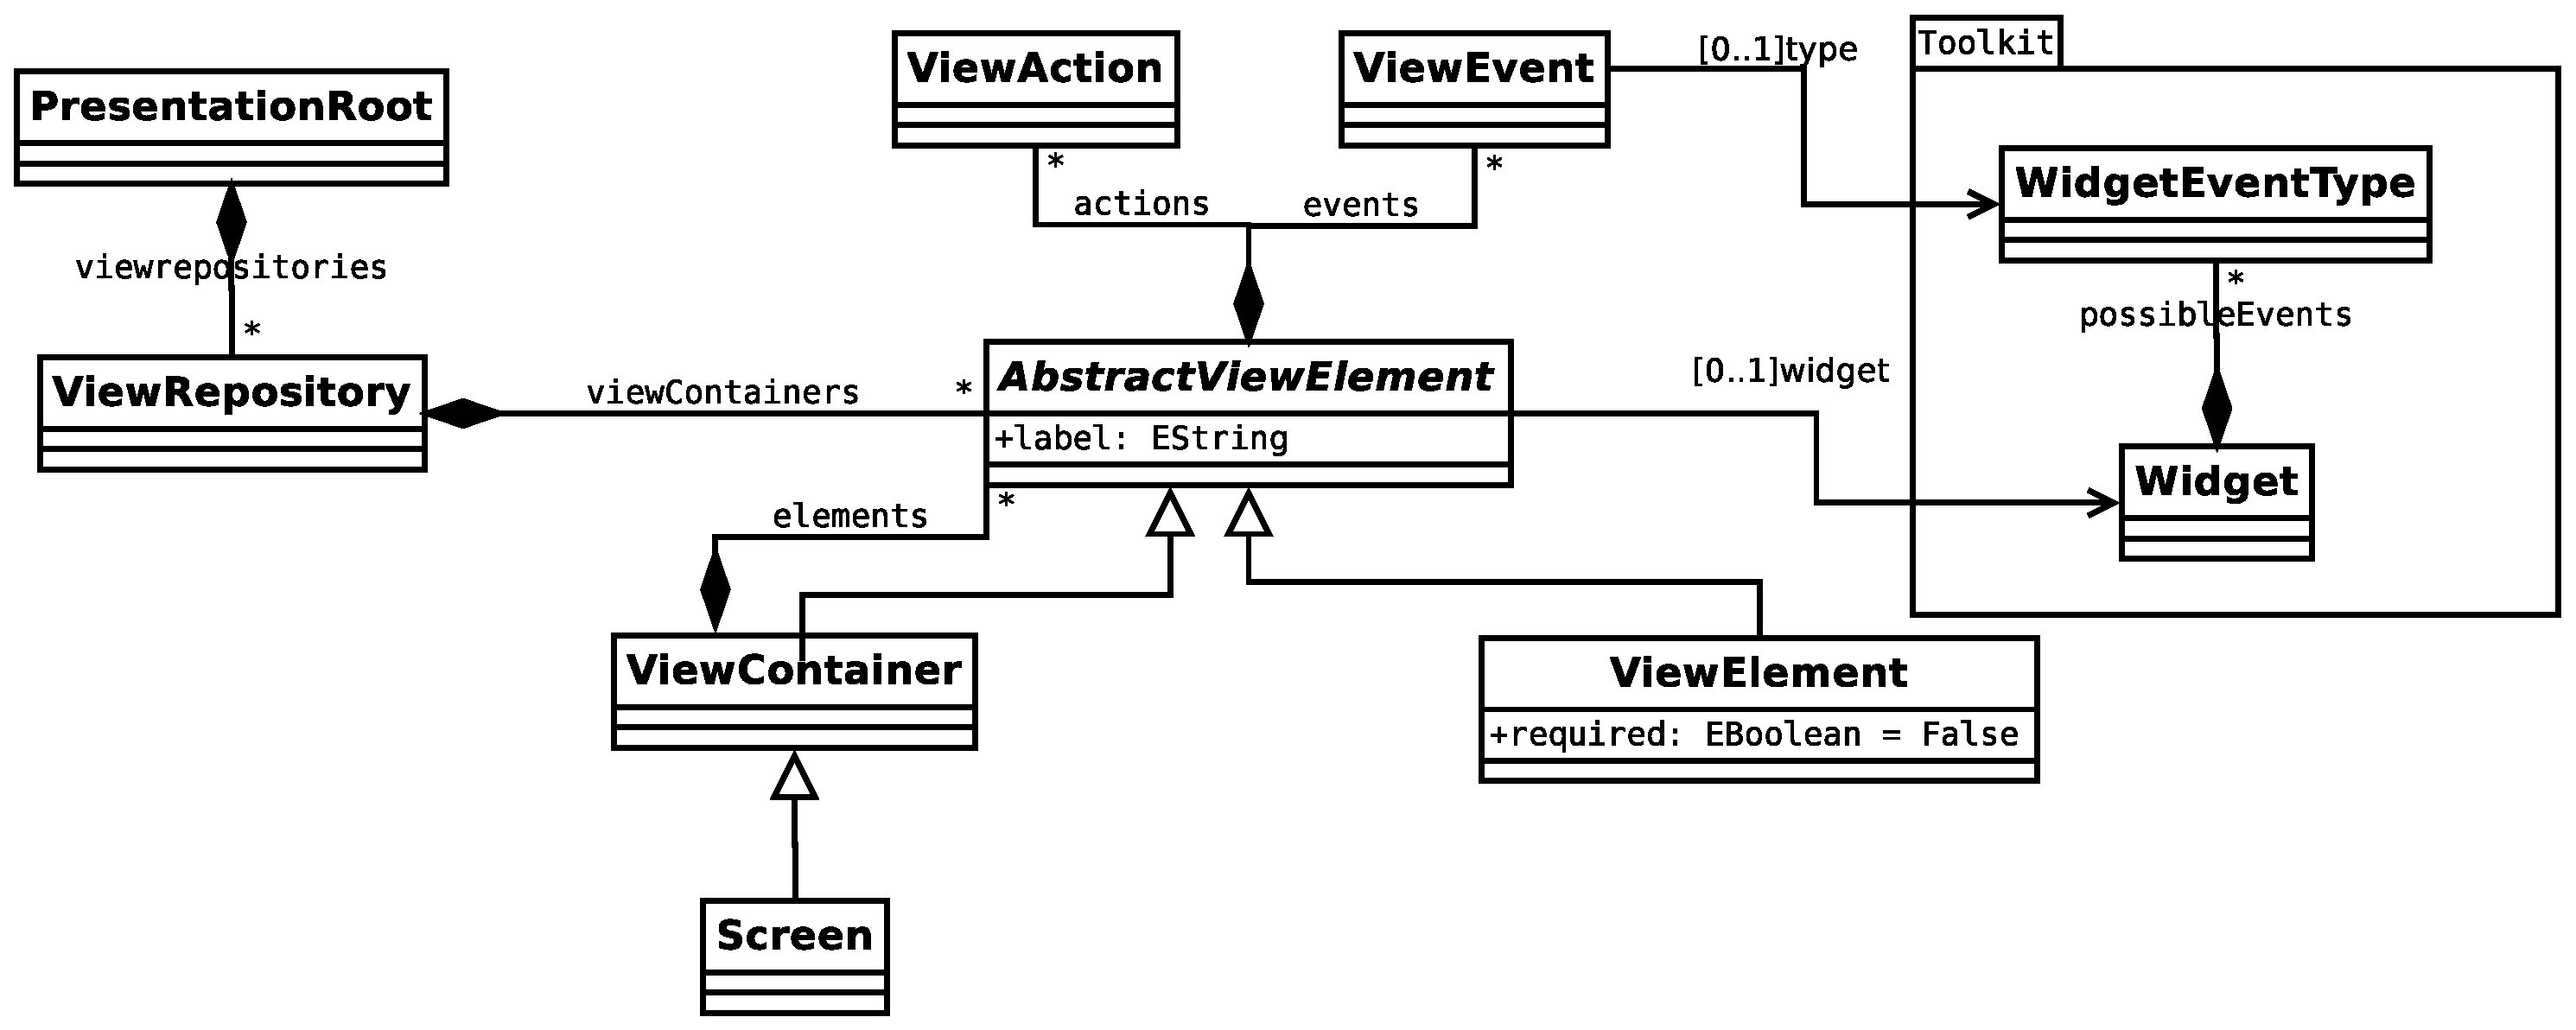
\includegraphics[scale=.3]{img/view.eps}
  \caption{Métamodèle view}
  \label{fig:view}
\end{figure}
  \item \textbf{Flow}: permet d'identifier le comportement dynamique des écrans \textsc{ihm}. Le flow peut être appréhendé comme une sorte de diagramme d'activités.

Le package Flow est illustré sur la figure \ref{fig:flow} :

\begin{figure}[H]
  \centering
  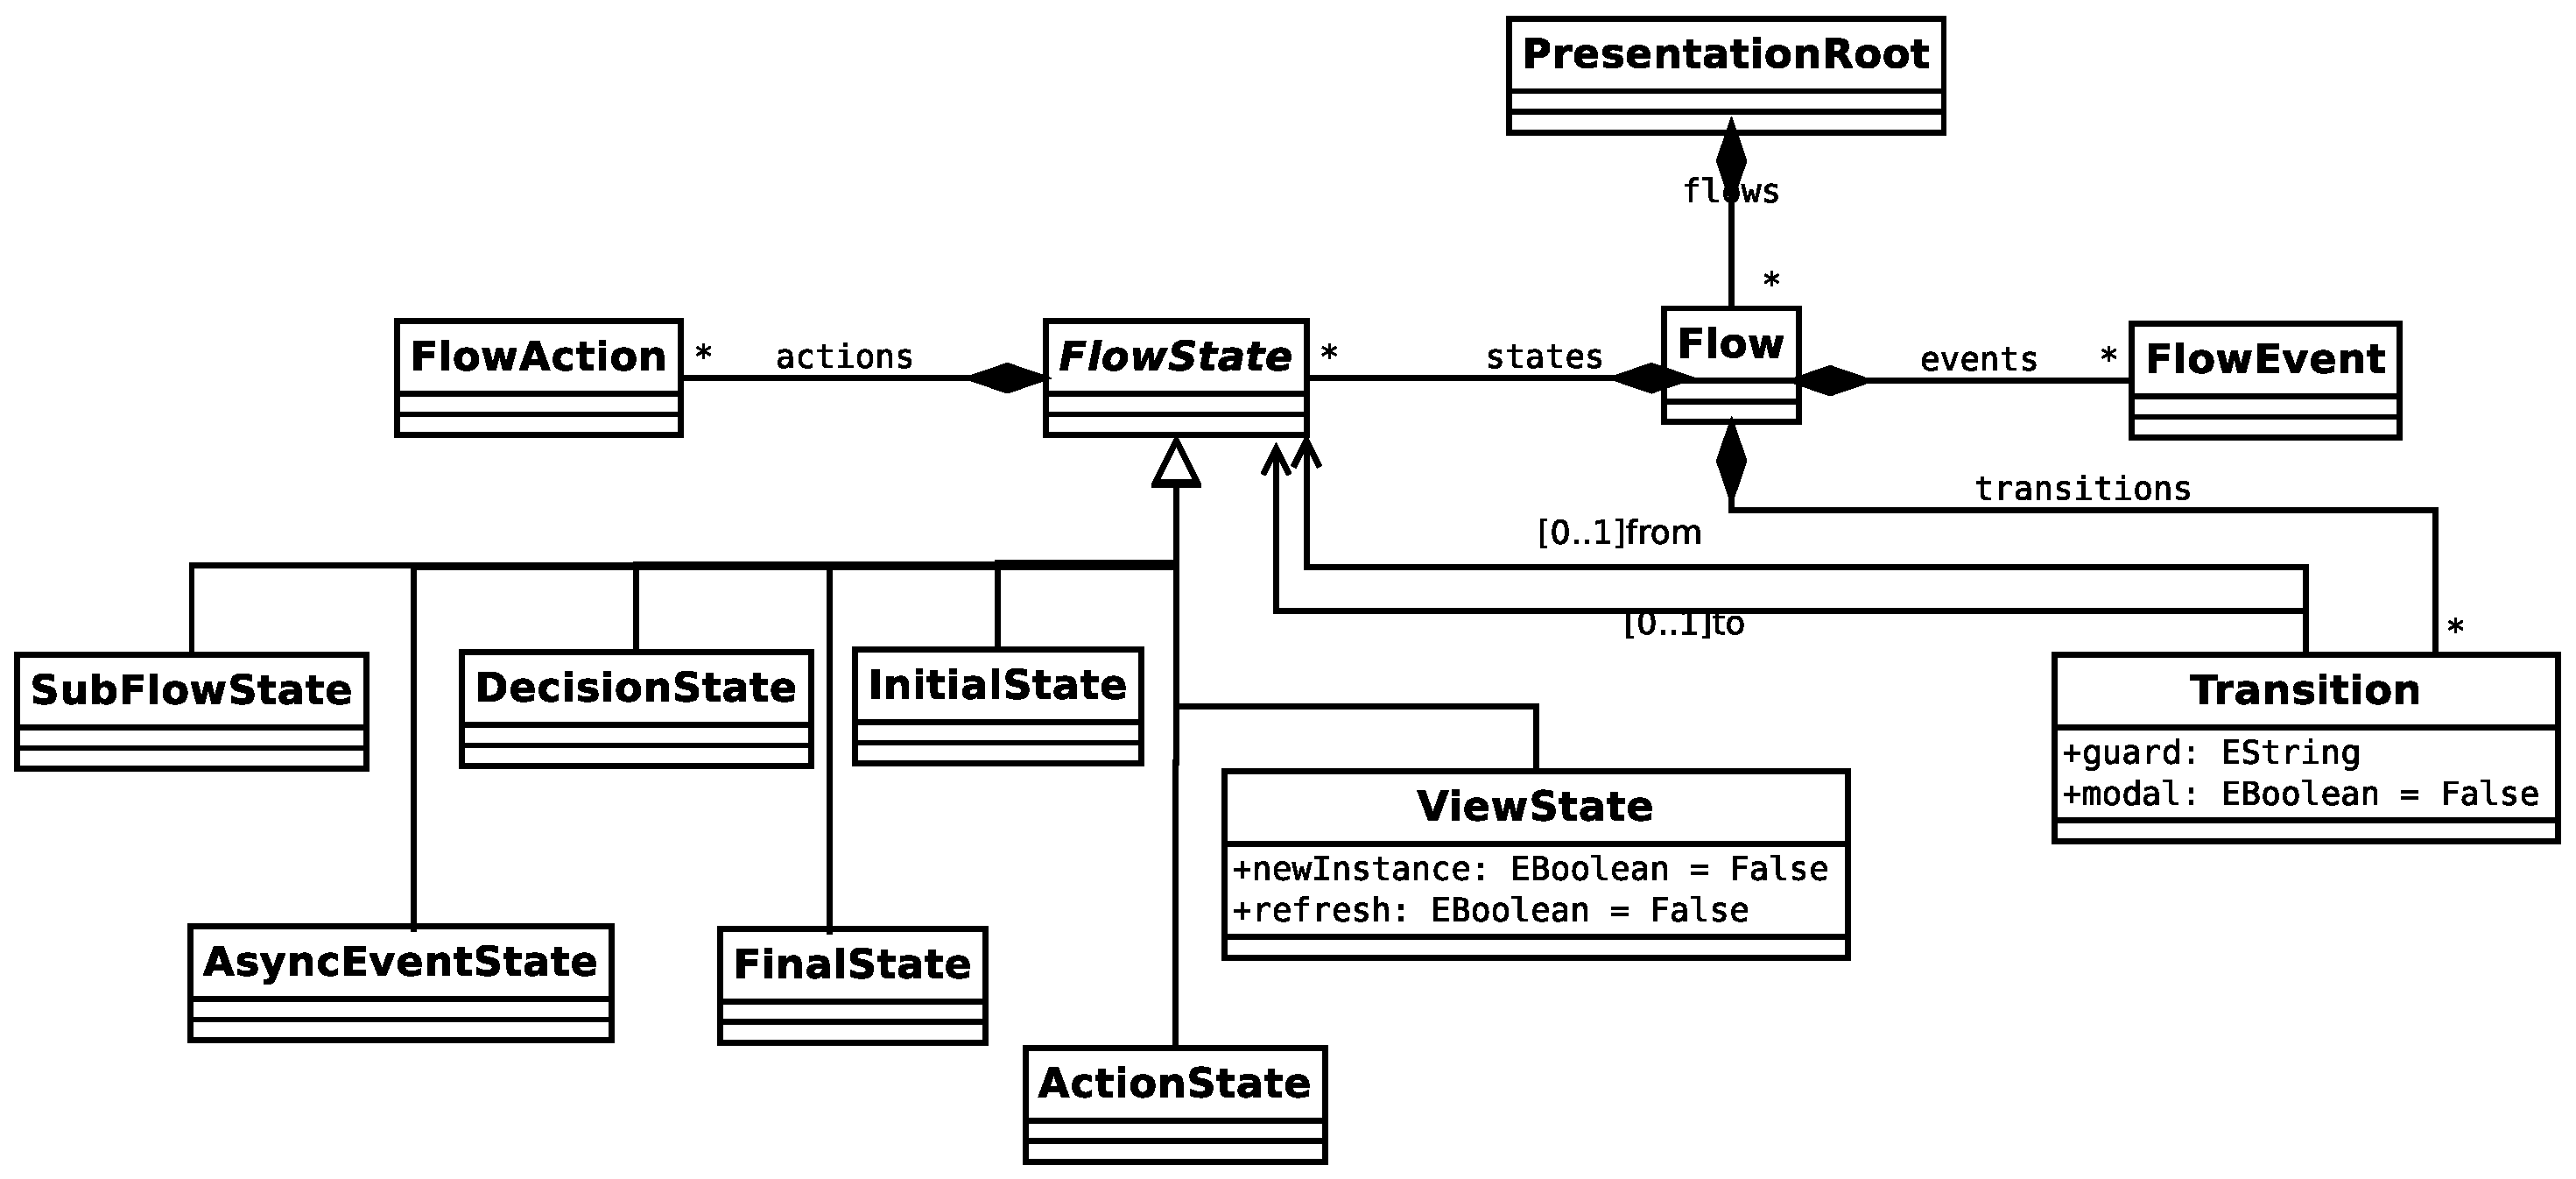
\includegraphics[scale=.3]{img/flow.eps}
  \caption{Métamodèle flow}
  \label{fig:flow}
\end{figure}

\end{itemize}


\subsection{Le concept cinématique dans \kwplay{}}
Nous retrouvons dans \kwplay{} un repertoire dans lequel sont regroupés les différents fichiers Web (HTML, XML,\dots) liés aux vues (principe MVC). Les fichiers relatifs à la création des \textsc{IHM} sont donc indépendants du reste de l'application.   

%%%%%%%%%%%%%%%%%%%%%%%%%%%%%%%%%%%%%%%%%%%%%%%%%%%%%
\subsection{Conception du modèle}
La modélisation \textsc{ihm} de l'application prototype \kwplay{} a été mise en place à l'aide de l'outil Acceleo. Le modèle est construit autour des trois principes du métamodèle défini précédemment:
\begin{enumerate}
\item \textbf{Toolkit}: Représente une palette contenant des widgets. Nous avons utilisé le modèle Toolkit (par défaut) car il couvre tous les éléments de type \guim{widget web}  actuellement existants (bouton, liste déroulante, champ de saisie, tableau, etc.). Chaque élément \guim{widget} peut lever des événements de type \textit{WidgetEventType} (\verb+onClick()+, \verb+onFocus()+ \dots). 

\item \textbf{View} : Permet de représenter tous les éléments graphiques d'une interface utilisateur. Au plus haut niveau, nous définissons les éléments de type \textit{View Container}. Un \textit{View Container} peut être de type \textit{Page}, \textit{Panel} (ou \guim{Formulaire}) ou \textit{Table}. 

Nous choisissons le type \textit{Page} pour représenter un écran \textsc{ihm}. Pour chaque \textit{ViewContainer} sont ensuite définis les éléments qu'il contient. Un élément peut être un formulaires, un tableau, ou encore un widget simples. Nos écrans sont alors construits de manière progressive jusqu'à obtenir toutes les fenêtres \textsc{IHM} qui composent l'application.
\begin{figure}[H]
  \centering
  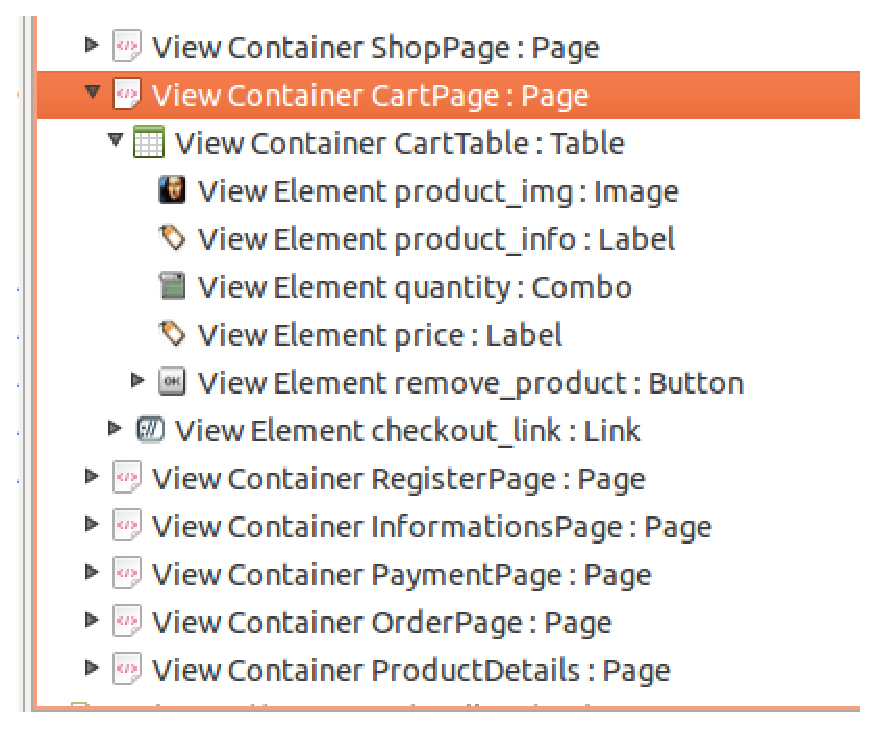
\includegraphics[scale=.4]{img/views.eps}
  \caption{Construction du modèle (partie Views)}
  \label{fig:view}
\end{figure}

\item \textbf{Flow} : Représente la manière dont les écrans de l'application peuvent s'enchaîner. Il décrit le comportement dynamique de l'\textsc{ihm} sous la forme d'enchaînements entre des états. Nous définissons ici, un état initial \textit{Initial State Start}, des états \textit{View State}, des états d'action \textit{Action State} et des transitions :
\begin{itemize}
\item Les états \textit{View State} correspondent aux écrans \textsc{ihm} et contiennent les \textit{View Container} décrit précédemment.
\item Les états d'action \textit{Action State} définissent les actions à réaliser sur chaque écran de l'application. Ils sont liés aux fonctions offertes par la partie \kwsoa{}. 
\textit{Exemple}: Pour le chargement de la liste des produits disponibles pour la page d'accueil (ou Vitrine), nous définissons un \textit{Action State} nommé \guim{Load Public Product List} que nous lions à l'opération getProductList() offerte par \kwsoa{}.  
\item Les transitions \guim{(\textit{Transition})} font passer l'\textsc{ihm} d'un état à un autre (d'un écran à un autre). Ils font également le lien entre les Action States et les View States. 
\paragraph{}
\textit{Exemple}: Une transition pour l'affichage de l'écran d'accueil \guim{Display Main Page} va de l'état \guim{Action State Load Public Product List} (chargement des éléments de la page \guim{Vitrine}) à l'état \guim{View State Display MainPage} (affichage de la page \guim{Vitrine}).
\newline
Les transitions peuvent également avoir des conditions de garde, déterminées par des View Events (elles n'occurrent ainsi que si les conditions d'activation sont remplies).
\end{itemize}
\end{enumerate}       
%%%%%%%%%%%%%%%%%%%%%%%%%%%%%%%%%%%%%%%%%%%%%%%%%%%%%%%%%%%%%%%%%%%%%%%%%%%%%%%%%%%%%%%%%%%%%%%%%%%


\subsection{Génération du code}
Dans cette partie, nous nous occupons de générer les fichiers relatifs aux \guim{routes}, aux \guim{controllers} et les \guim{views}. Rappelons les caractéristiques de chaque type de fichier:
\begin{itemize}
\item \textbf{Controller}: Nous avons une classe \guim{MainController} dans laquelle sont déclarées des méthodes statiques pour chacune de nos Actions;
\item \textbf{Route}: Fichier de configuration des routes au sein de l'application. Les \guim{routes} sont toutes associées au même controleur : \guim{MainController}. 
\item \textbf{View}: Ensemble de fichiers décrivant un moteur de templates qui repose entièrement sur Scala ainsi que du code html pour la définition des formulaires, widgets, etc. 
\end{itemize}
Le Générateur \guim{Cinematic} se divise ainsi en un fichier de génération principal, GenerateCinematic, lié aux fichiers de génération majeurs (un pour chaque type de fichiers - Controller, Route, View), eux-même appelant des fichiers secondaires comportant les templates et queries nécessaires à l'élaboration des fichiers finaux en Scala et HTML.
\begin{figure}[H]
  \centering
  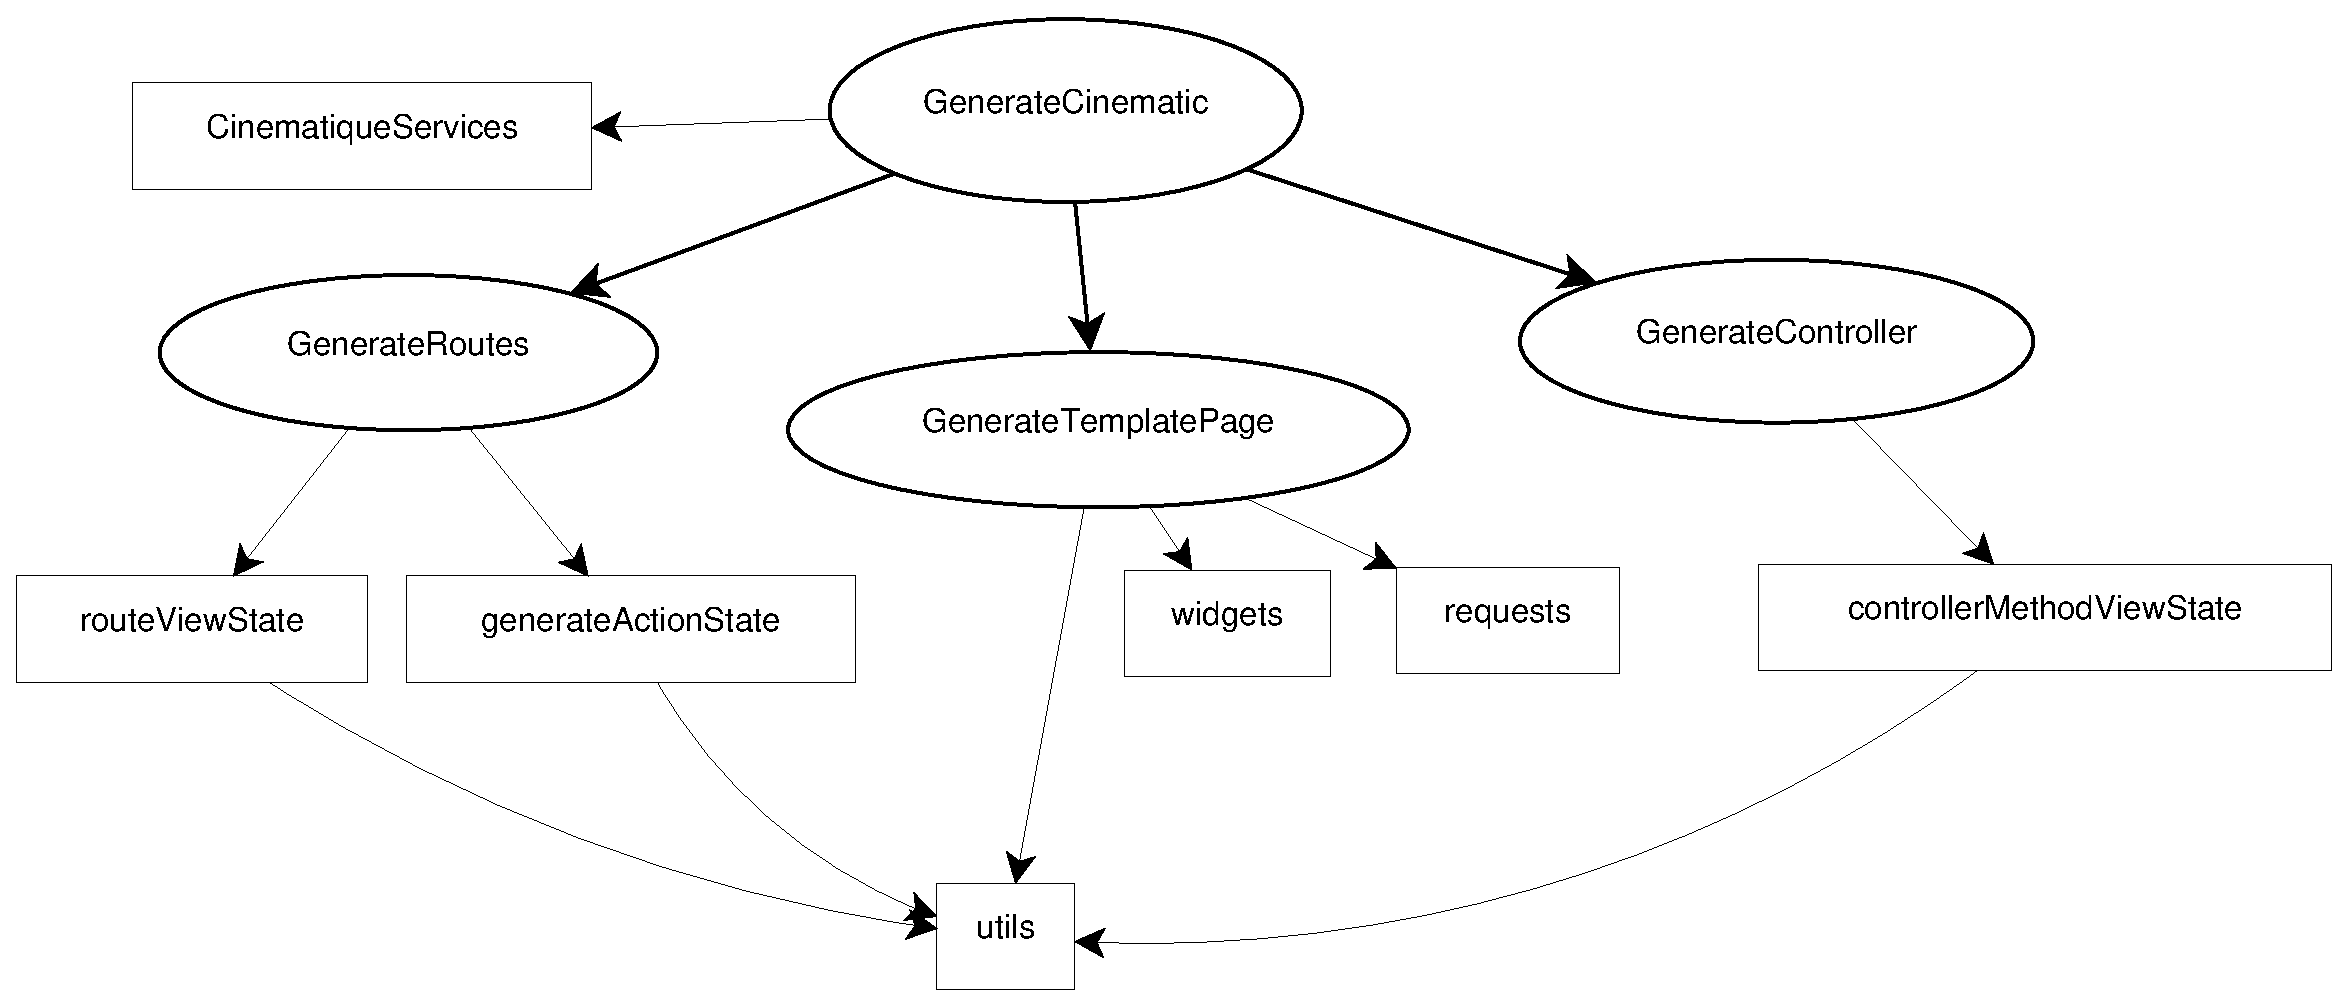
\includegraphics[scale=.35]{img/hierarchie.eps}
  \caption{Hierarchie des fichiers générateurs. Chaque ellipse correspond à un générateur \guim{principal}, et chaque rectangle à un fichier de templates secondaire.}
  \label{fig: hierarchie generateurs}
\end{figure}
A partir d'un Modèle composé comme décrit précédemment, le Générateur va analyser chacun de ses éléments et, à l'aide des templates correspondants, les traduire afin de créer les fichiers Scala/HTML finaux. 
\\
\textbf{Le générateur de Routes} analysera le Flow principal du modèle, et traduira chaque ViewState et ActionState en appels vers des méthodes contenues dans le Controller.
\\
De même, \textbf{le générateur de Controller} générera, pour chaque ViewState du même Flow, l'ensemble des méthodes lui étant associées - ces mêmes méthodes mentionnées dans les Routes.
\\
\textbf{Le générateur de Views} permet la création des différentes pages de l'application - le modèle entier est analysé afin de permettre la création de chacun des éléments nécessaires à l'IHM. Une application Scala est composée d'une page principale, dite \guim{main} ou \guim{index}, qui fait appel à d'autres pages qui correspondent aux différents écrans de l'application. Ainsi, la page \guim{index}, indépendante des autres écrans, n'est pas représentée dans le modèle - elle est cependant générée automatiquement avant la génération des écrans.
\\
Chaque page est décrite au sein d'un ViewState (écran) par l'intermédiaire d'un ViewContainer de type \guim{Page}. Dans notre modèle actuel, il est supposé qu'un ViewState ne contient qu'un seul ViewContainer de type \guim{Page} (un écran = une page). De cette manière, un seul fichier de vue HTML est créé par ViewState, et donc par écran. Le ViewContainer \guim{Page} peut contenir à son tour soit d'autres ViewContainers, soit des ViewElements (qui représentent des Widgets). Par exemple, les \guim{Tables} et les \guim{Formulaires} sont des conteneurs. Le rôle du générateur de Views est de traduire chacun de ces éléments en code HTML pour chaque écran.
\\
Toute page du modèle est créée selon les étapes d'analyse d'élément suivantes :
\begin{enumerate}
\item CinematicRoot (le modèle) : récupération et analyse de chaque ViewState tour à tour.
\item ViewState : récupération du ViewContainer \guim{Page} correspondant à l'écran souhaité.
\item ViewContainer \guim{Page}: récupération et analyse de chaque élément contenu (ViewContainers secondaires ou ViewElements).
\item ViewContainer secondaire : \guim{Table} ou \guim{Panel} - traduction du conteneur dans les fichiers finaux (création de formulaire ou de tableau html), et analyse des ViewElements qu'il contient.
\item ViewElement : traduction de chaque type de ViewElement en widget Scala/HTML dans les fichiers finaux (création de champs de saisie, de boutons...).
\end{enumerate}
Plutôt que de créer un template par type d'élément, nous avons créé des templates \guim{conditionnels}. Ainsi, par exemple, pour la génération de ViewElements, un seul Template est appelé - cependant, selon la nature du ViewElement (déterminée par une Query), une seule des spécifications du Template sera mise en oeuvre. Il en est de même pour les ViewContainers secondaires. De cette façon, un code \guim{personnalisé} pour chaque élément est généré, prenant en compte le type de l'élément, son environnement (conteneur) et ses propriétés (label...).
\newline
\begin{figure}[H]
  \centering
  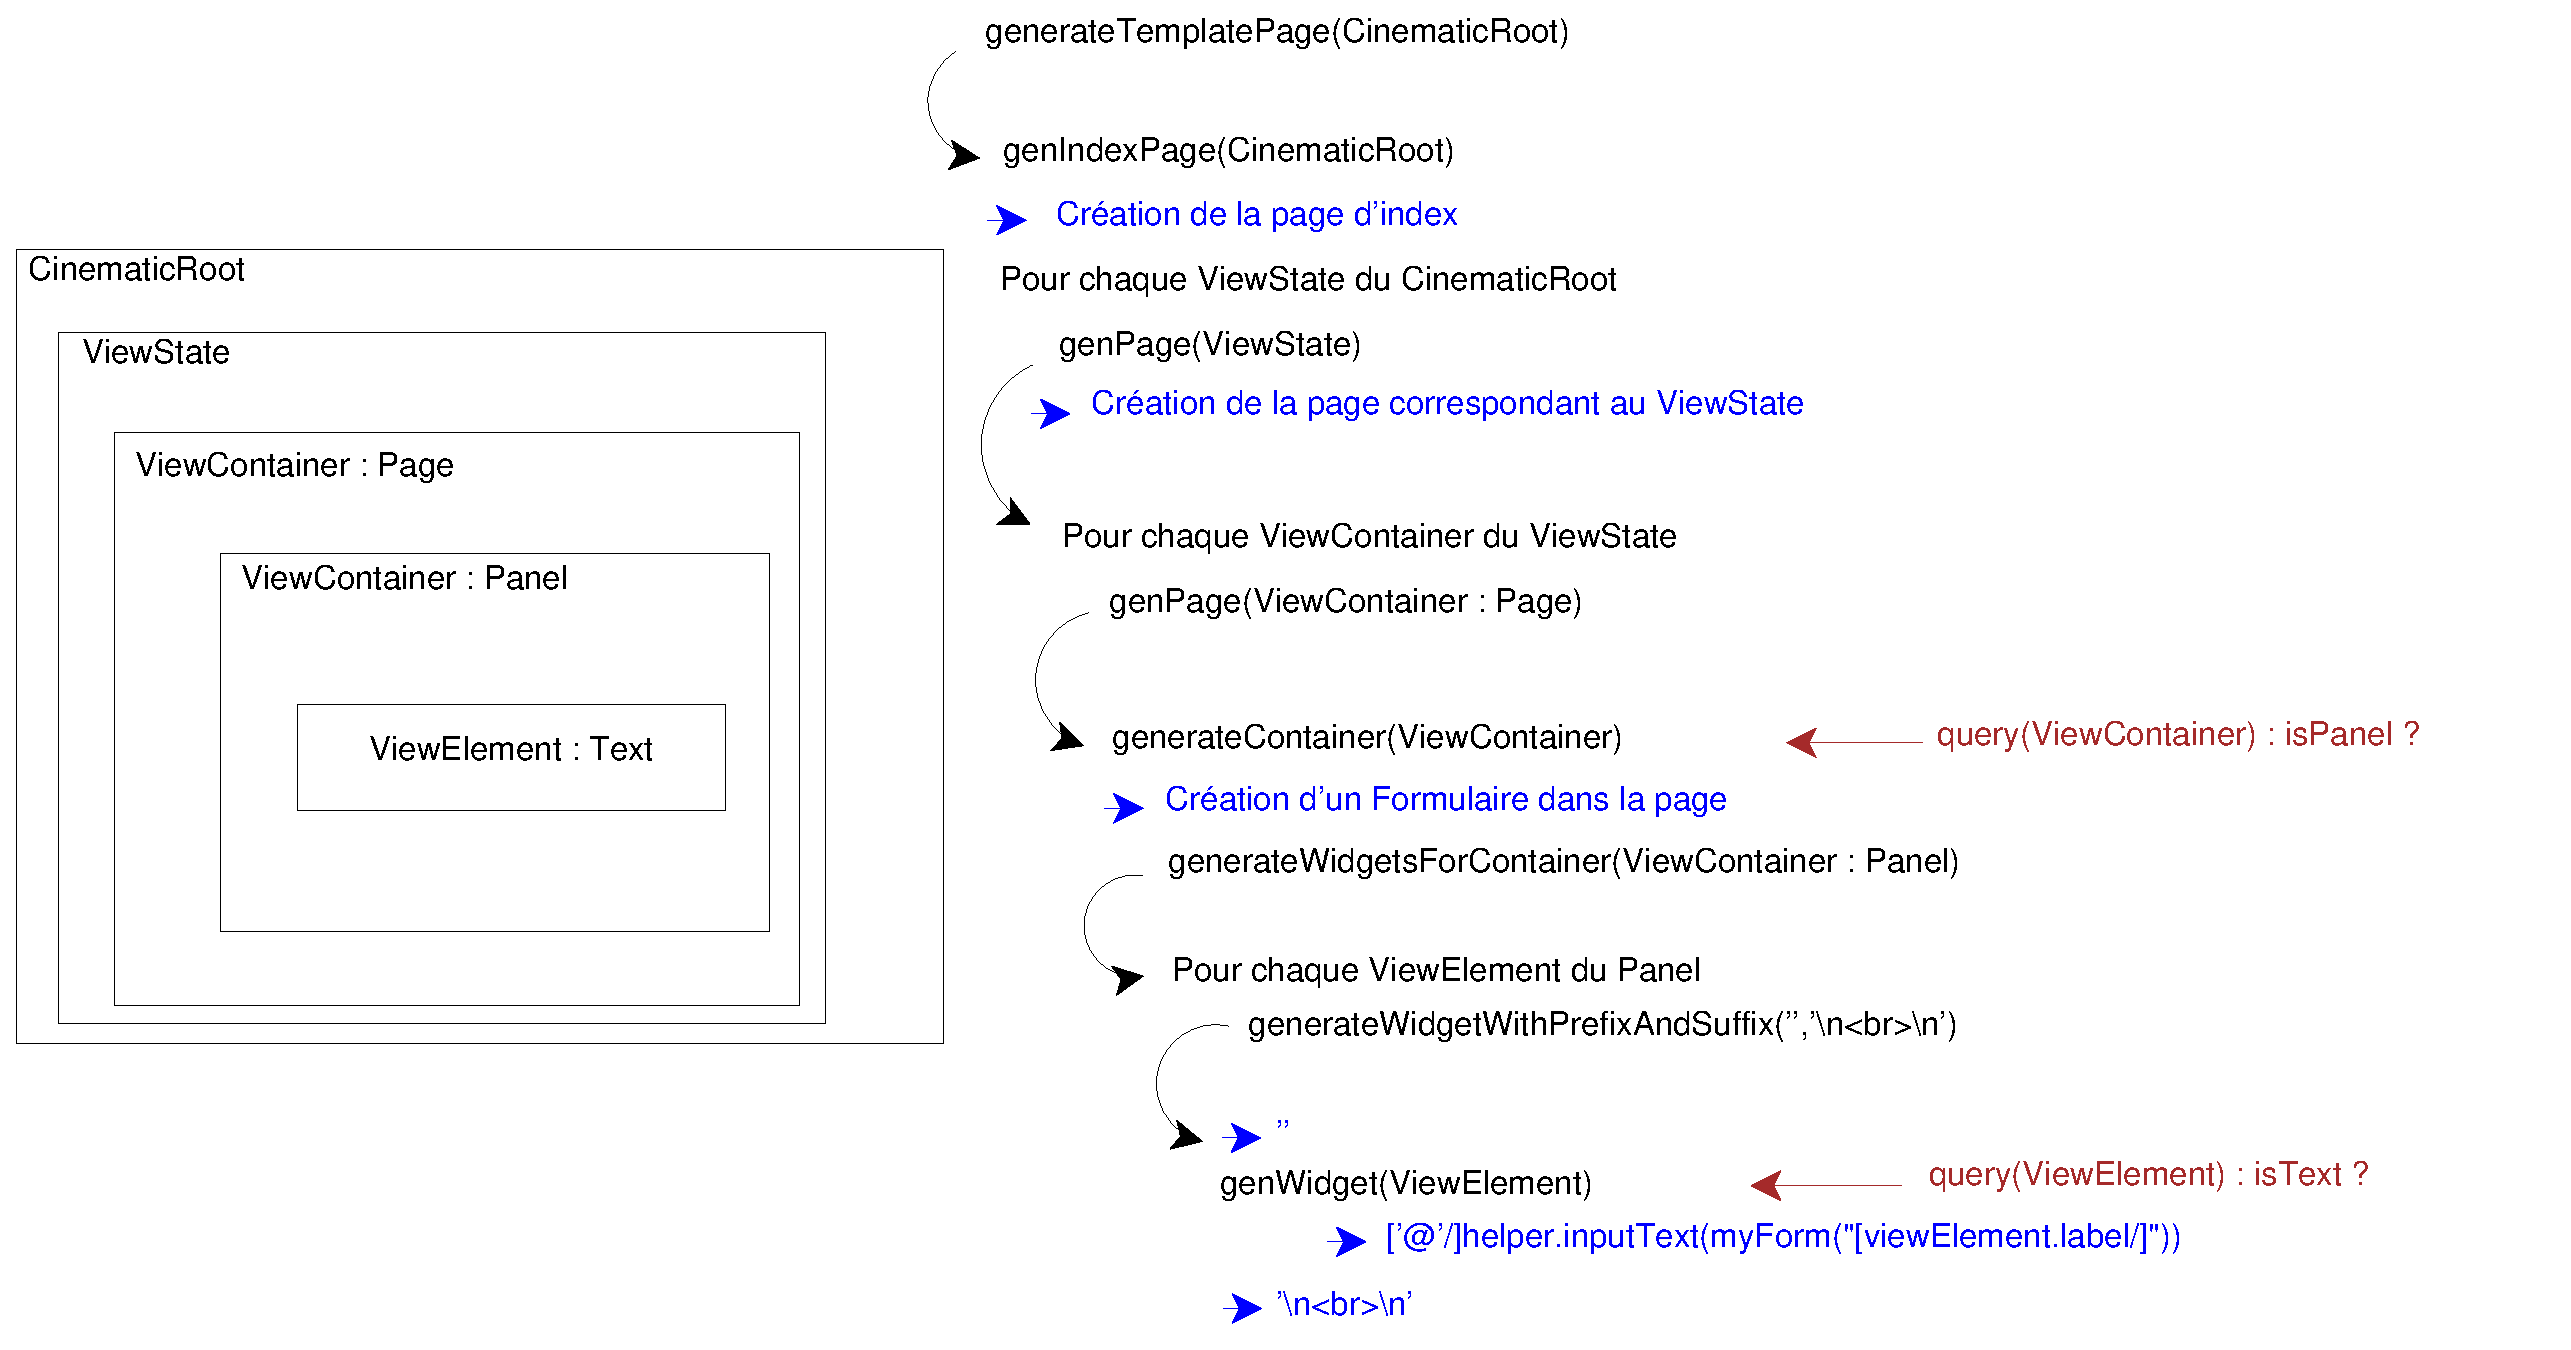
\includegraphics[scale=.35]{img/viewexample.eps}
  \caption{Exemple d'analyse par le générateur de views.}
  \label{fig: exemple generateur view}
\end{figure}
\paragraph{Actions}
Certains éléments, tels que les formulaires et les boutons, requièrent des déclencheurrs d'Actions (envoi de données par exemple). La nature de ces Actions ne peuvent être récupérées directement à partir d'un élément d'un ViewContainer : Il faut utiliser les Transitions afin de savoir si un évènement ou une vue est reliée à une Action.

De l'élément du ViewContainer analysé, il peut se trouver un ViewEvent (évènement tel qu'un clic sur un Bouton). Cet évènement est unique, spécifique à cet élément. On peut alors parcourir le Flow principal, afin de vérifier si une des Transitions prend sa source de cet Évènement. Si une telle transition existent et que sa cible est un ActionState, il est alors possible de récupérer l'Operation associée (définie dans le Modèle \kwsoa). Il est ainsi possible de lier un Évènement à une Action, et il suffit alors de générer l'appel de l'Opération correspondante (en utilisant le système de Routes).

\subsection{Le cas du \guim{Header}}
Si l'utilisateur veut créer un \guim{Header} (en-tête de page) visible sur toutes les pages, et présentant des liens vers différentes pages de son application, il n'est pas concevable que ce dernier soit forcé d'ajouter la description de ce \guim{Header} dans toutes les Pages du Modèle. Le système que nous avons mis en place propose plusieurs solutions à ce problème : L'utilisateur peut modifier son Modèle de telle sorte que les pages à référencer soient mises en valeur, avec un attribut spécial par exemple. (TODO)
